\documentclass[12pt,a4paper]{book}

% Formato del documento
\usepackage[papersize={210mm,297mm},inner=3.5cm,outer=2cm,top=2.5cm,bottom=2.5cm]{geometry}
\renewcommand{\baselinestretch}{1}
\setlength{\parskip}{8pt}

\usepackage[utf8]{inputenc}
\usepackage{amssymb}
\usepackage{amsmath}
\usepackage{graphicx}
\usepackage{tikz}
\usepackage{tkz-graph}
\usepackage{hyperref}
\usepackage[parfill]{parskip}
\usepackage{float}

\renewcommand{\chaptername}{Capítulo}
\renewcommand{\contentsname}{Índice}
\renewcommand{\bibname}{Bibliografía}
\renewcommand{\figurename}{Figura}

\definecolor{verde_oscuro}{rgb}{0.0, 0.5, 0.0}

\newtheorem{defi}{Definición}[section]
\newtheorem{prop}{Proposición}[section]
\newtheorem{propi}{Propiedades}[section]
\newtheorem{lema}{Lema}[section]
\newtheorem{tma}{Teorema}[section]
\newtheorem{cor}{Corolario}[section]
\newtheorem{nota}{Nota}[section]
\newtheorem{ejem}{Ejemplo}[section]

\hypersetup{
    colorlinks=true,
    linkcolor=blue,
    filecolor=magenta,      
    urlcolor=cyan,
    pdftitle={Overleaf Example},
    pdfpagemode=FullScreen,
    }

\urlstyle{same}

% Cabecera
\usepackage{fancyhdr}
\pagestyle{fancy}
\fancyhf{}
\renewcommand{\chaptermark}[1]{\markboth{\textbf{Cap\'itulo \thechapter}}{}} 
\fancyhead[LO]{Cap\'itulo \thechapter \quad P\'agina \thepage}
\fancyhead[RO,LE]{\textbf{\thepage}}

%%%%%%%  Comando Portada  %%%%%%%%%%%
\newcommand{\nuevaportada}[6]{
    \thispagestyle{empty}
    \begin{center}
        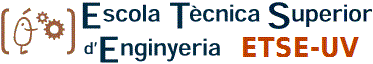
\includegraphics[width=0.5\textwidth]{images/logo.png}
        
        \vspace{0.5cm}
        {\Large\bfseries\textsc{M\'aster Universitario en #1}\par}
        
        \vspace{0.5cm}
        
\includegraphics[width=0.4\textwidth]{images/uv.png}
        
        \vspace{0.5cm}
        {\Large\bfseries\textsc{Trabajo de Fin de M\'aster}\par}
        
        \vspace{0.5cm}
        {\Large\bfseries #2\par}
        
        \vspace{2cm}
        \begin{flushright}
            \begin{tabular}{l} 
                {\large\bfseries\textsc{Autor:}} \\
                {\large\textsc{#3}} \\ [0.5cm] 
                {\large\bfseries\textsc{Tutora:}} \\ 
                {\large\textsc{#4}} \\ [0.5cm]
                {\large\bfseries #5} 
            \end{tabular}
        \end{flushright}
    \end{center}
    \clearpage
}

\begin{document}

\frontmatter
\pagenumbering{gobble}
\nuevaportada{Ciencia de Datos}{Algoritmo para el Problema de Localización de Centros k-Balanceado Multiobjetivo}{Manuel Rubio Martínez}{Anna Martínez Gavara}{Abril, 2025}

\clearpage
\thispagestyle{empty} \mbox{} \clearpage

\newpage
\tableofcontents

\chapter{Introducción}

El comienzo del estudio de los grafos se remonta a una época no tan lejana, donde el famoso Euler, a mitades del siglo XVIII planteaba el famoso problema
de los puentes de Königsberg. Esta teoría ha ido evolucionando, hasta hoy en día. Unas de las principales aplicaciones son: poder optimizar rutas de transporte, difundir información, en ciencia de datos
para algunos de sus algoritmos, etc. 

\smallskip

En este trabajo, comenzaré resolviendo un par de juegos que, resultarían más complicados resolverlos a mano, pero que utilizando grafos la solución se vuelve sencilla. Para continuar, hablaré sobre
formas concretas de recorrer grafos, en concreto cómo salir de laberintos, o hacer que no nos perdamos en ellos. Para terminar con esta primera parte, demostraré un algoritmo que encuentra el camino más corto
entre cualquier par de puntos de un grafo, y cómo se puede implementar en uno de los juegos que anteriormente resolvimos.

\smallskip


A continuación, en la segunda parte hablaré de un matemático no tan conocido en este ámbito, como es Paul Turán, y su estudio en la teoría de grafos extremales. Esta teoría consistente en, dado un grafo de un determinado número de vértices, ver cuál es
el mayor número de aristas que puede tener, sin contener ciertos subgrafos. Por ejemplo, 


\chapter{Preliminares}
\section{Conceptos básicos de la teoría de grafos}

\begin{defi}
Un \textbf{grafo} $G$ es una estructura formada por un par $G=(V,E)$ donde $V$ es el conjunto de vertices, el cual
tiene que ser no vacío y finito, y $E$ es un conjunto de pares no ordenados de elementos . A los elementos
de $V$ se les llama \textbf{vértices} o \textbf{nodos} y a los elementos de $E$ se les llama \textbf{aristas}.

\smallskip

Si una arista está compuesta por 2 elementos iguales, se dice que es un \textbf{lazo}.

\end{defi}
\bigskip

\chapter{Modelo Matemático}


\chapter{Grasp}




\chapter{Experimentación y Resultados}


\chapter{Conclusiones}





\begin{thebibliography}{X}
    \bibitem{Juegos} \textsc{Martín Novo, Eduardo; Méndez Alonso, Alfredo}.
    \textit{Aplicaciones de la teoría de grafos a algunos juegos de estrategia.}
    \url{https://redined.educacion.gob.es/xmlui/handle/11162/13874}

    \bibitem{Caníbales} Caníbales y misioneros: \url{https://culturacientifica.com/2016/05/04/problema-los-tres-caballeros-los-tres-criados/}

    \bibitem{Laberintos} Laberintos: \url{https://www.cantab.net/users/michael.behrend/repubs/maze_maths/pages/tarry_lab_en.html}
    
    \bibitem{Ajedrez} Sobre ajedrez: \url{https://chess24.com/es/informate/noticias/como-piensan-y-operan-los-modulos-de-analisis}

    \bibitem{Mantel} Teorema de Mantel: \url{https://lidicky.name/oldteaching/20.569X/l13%20-%20Mantel.pdf}

    \bibitem{Turan} Vascimini, Vincent. (2017). Extremal Graph Theory: Turán’s Theorem. 
    In BSU Honors Program Theses and Projects. Item 234. Available at: \url{https://vc.bridgew.edu/honors_proj/234}

    \bibitem{otros_teoremas} \textsc{Widdershoven, Cas.} \textit{Extremal graphs and the Erd{\H{o}}s-Stone-Simonovits theorems.}
    \url{https://studenttheses.uu.nl/handle/20.500.12932/23972}

\end{thebibliography}


\end{document}

